\begin{frame}[plain,c]
%\frametitle{A first slide}

\begin{center}
\Huge Backup
\end{center}

\end{frame}

\begin{frame}{Evolutionary neural networks}
    \begin{itemize}
        \item Starting with a set of random configurations
        \vspace{0.2cm}
        \item Evaluate the results of the first generation and generate a new generation based on AUC 
        \vspace{0.2cm}
        \item Repeat until a good configuration is reached
        \vspace{0.2cm}
        \item Advantages:
            \begin{itemize}
                \item Decrease user bias for hyperparameter choice
                \item Optimised to run on worker nodes
                \item Quick discarding of bad configurations
                \item User friendly for unexperienced students
            \end{itemize}
    \end{itemize}
\end{frame}

%\begin{frame}{Inner product}
%    \begin{equation*}
%        a^{\mu} = \begin{pmatrix}
%            p_T \cosh ( \eta ) \\
%            p_T \cos ( \phi ) \\
%            p_T \sin ( \phi ) \\
%            p_T \sinh ( \eta ) \end{pmatrix}
%    \end{equation*}
%    %
%    \begin{align*}
%        \langle A | B \rangle = A_{\mu} B^{\mu}\\
%        = p_{T,A} p_{T,B} ( \cosh ( \eta_A ) \cosh ( \eta_B ) - \cos ( \phi_A ) \cos ( \phi_B)\\
%        - \sin ( \phi_A ) \sin ( \phi_B ) -\sinh ( \eta_A ) \sinh ( \eta_B ) )\\
%        = p_{T,A} p_{T,B} \left( \cosh ( \eta_A - \eta_B ) - \cos ( \phi_A - \phi_B ) \right)
%    \end{align*}
%\end{frame}

\begin{frame}{Responses}
  \begin{columns}
    \begin{column}{0.5\textwidth}
      \begin{figure}
      \centering 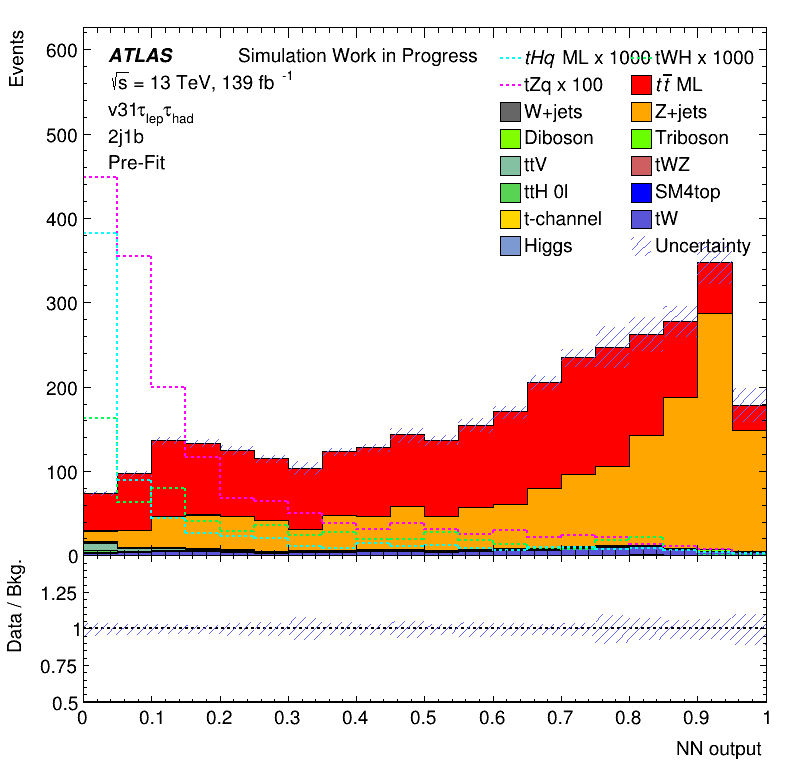
\includegraphics[width=\textwidth]{response_bkg}
      \caption{Background response}
      \end{figure}
    \end{column}
    \begin{column}{0.5\textwidth}
      \begin{figure}
      \centering 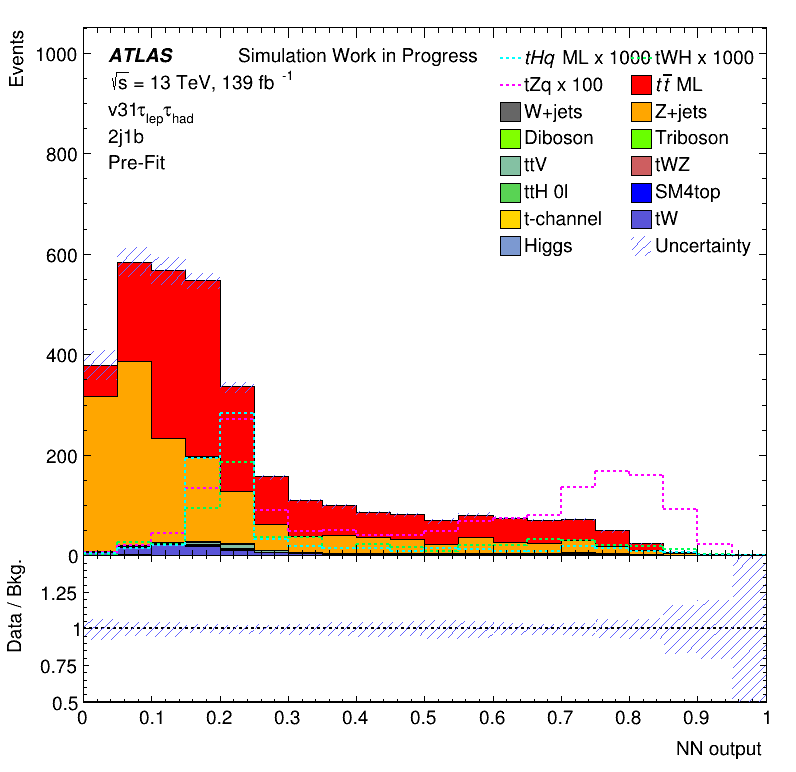
\includegraphics[width=\textwidth]{response_tZq}
      \caption{\tZq response}
      \end{figure}
    \end{column}
  \end{columns}
\end{frame}

\begin{frame}{\tHq versus \tZq}
  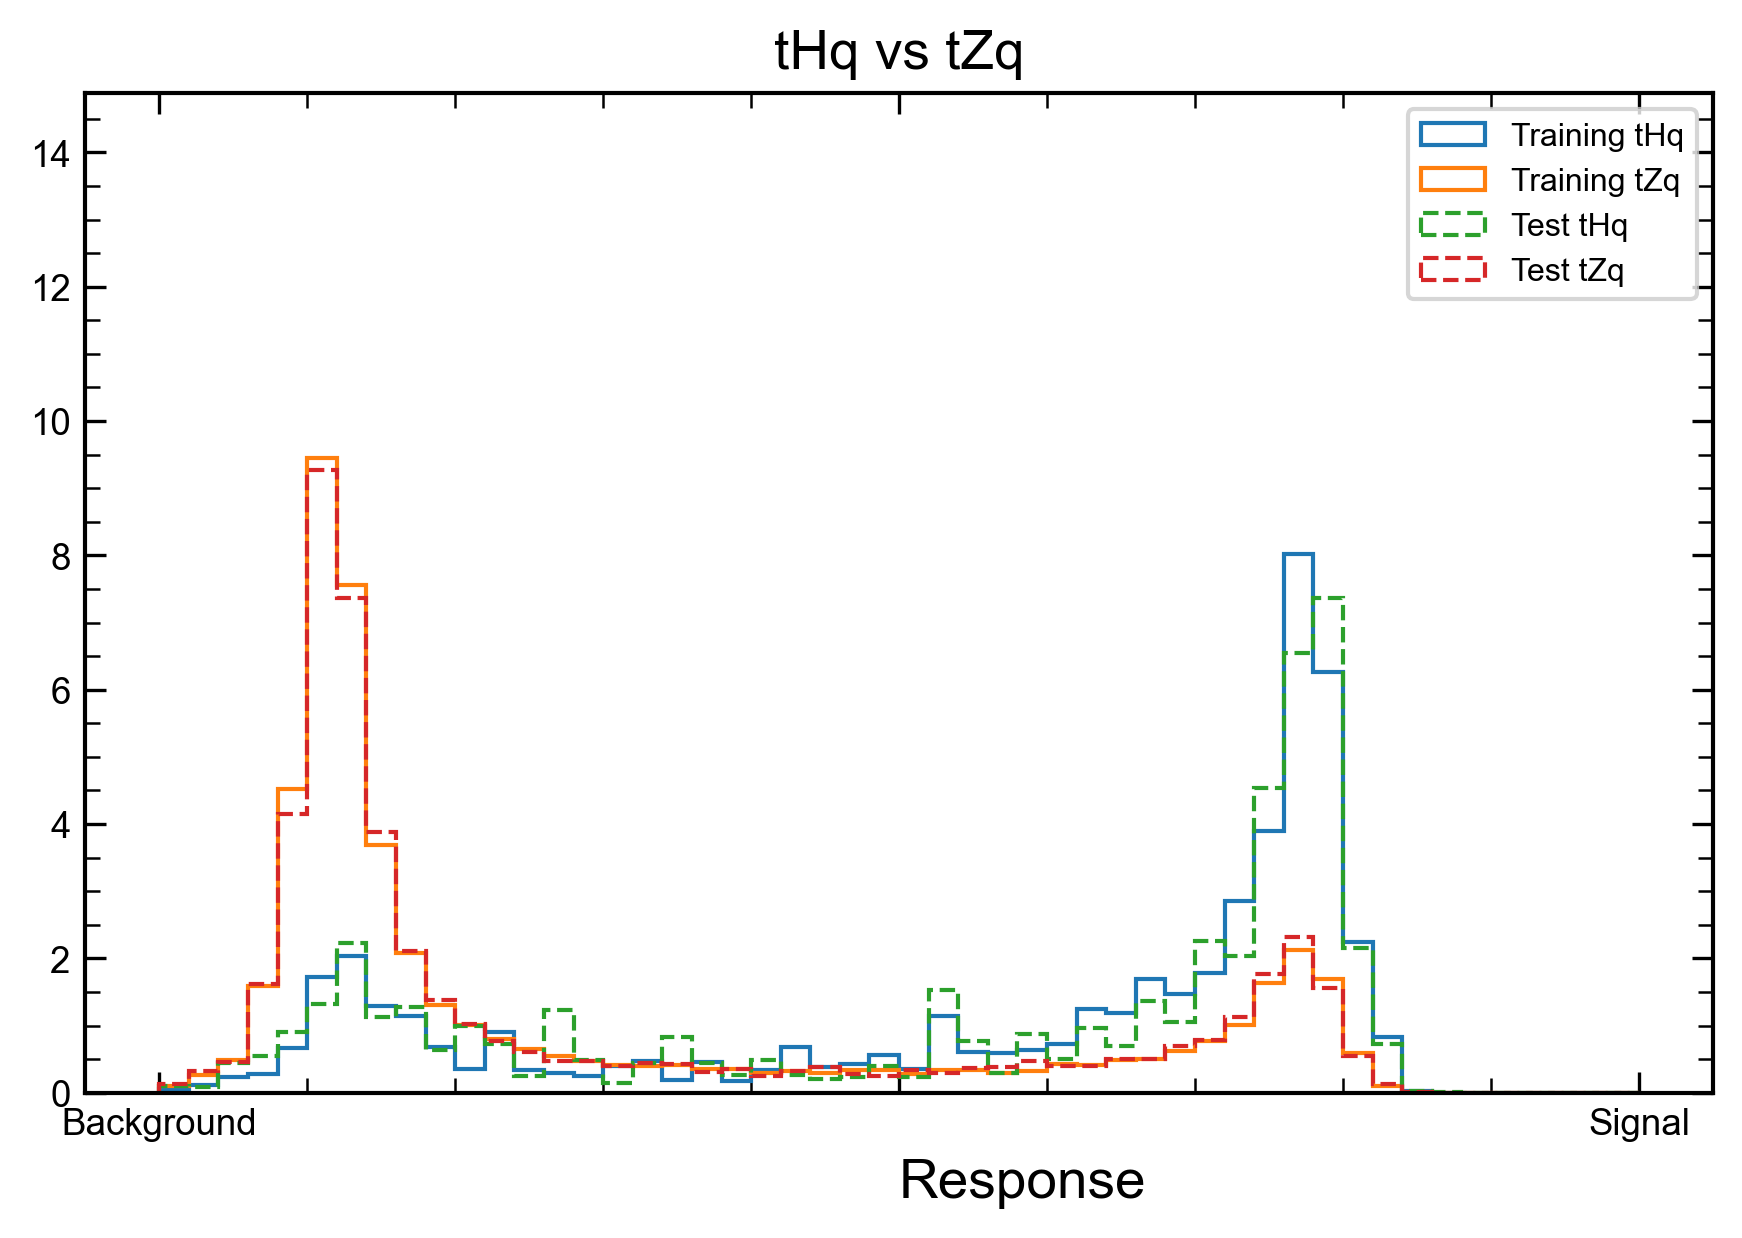
\includegraphics[width=\textwidth]{tHqvstZq.png}
\end{frame}

\begin{frame}{BDT summary}
    \begin{itemize}
        \item {\large A cut a bit below 0.2 would remove around 99\% of bkg
            events and 80\% of signal. Having just the 1\% of the bkg
            and 20\% of the signal would greatly increase our
            significance.}
        \vspace{0.2cm}
        \item {\large With the cut on the BDT we would have (approx.): bkg/sg = 4877/20 = 243
              Improved by a factor 71 to the before-presel scenario. Including BDT score in the trees}
        \vspace{0.2cm}
        \item {\large Using all events, not just the ones with positive weights reduces AUC surprisingly significantly}
        \vspace{0.2cm}
        \item {\large In the future the BDT should be tested in specific regions or for specific backgrounds}
    \end{itemize}
\end{frame}

\begin{frame}{}
  \centering 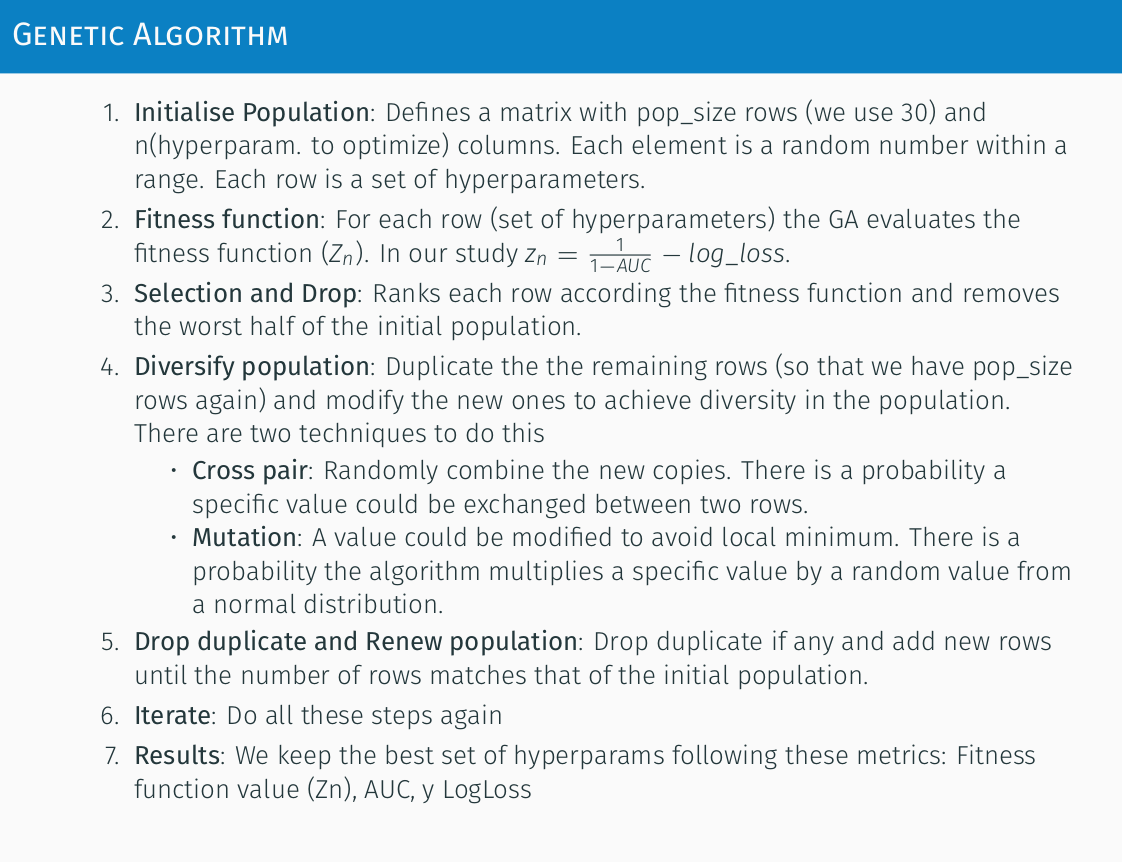
\includegraphics[width=\textwidth]{geneticAlg}
\end{frame}
